\documentclass[pageno]{jpaper}

% Change to current semester and year, e.g.:
% \newcommand{\IWreport}{Spring 2020}
\newcommand{\IWreport}{Fall 2020}
\newcommand{\quotes}[1]{``#1''}

\widowpenalty=9999

\usepackage[normalem]{ulem}
\usepackage{caption}
\usepackage[newfloat]{minted}
\usepackage{keystroke}
\captionsetup[listing]{position=top}

\begin{document}

\title{Improving the Marching Cubes Algorithm for Use in Deformable 3D Terrain}

\author{William Svoboda\\Adviser: Szymon Rusinkiewicz}

\date{}
\maketitle

\thispagestyle{empty}
\doublespacing
\begin{abstract}
Procedural generation can create endless virtual worlds without human intervention. However, prevailing methods for rendering these worlds lack realism. The marching cubes algorithm~\cite{lorensen} offers an alternative solution that produces more detailed results overall. This paper describes an implementation of the algorithm to create deformable 3D terrain in real-time. The problem of terrain generation is contextualized within the extraction of an isosurface from a scalar field, and interactive enhancements to marching cubes are discussed.
\end{abstract}

\section{Introduction}

The natural world is both enormous in size and fine in detail. While a perfect digital recreation of the universe might be ideal, computers are limited in their power and memory. Some way of approximation, therefore, is required to create virtual environments that are convincing. It is likely that this problem has been around for as long as computation itself has existed, and it remains an area of active development. The popular video game Minecraft (Mojang 2009) uses voxels as the core of its 3D environment. As Figure \ref{fig:minecraft} illustrates, Minecraft features large, procedurally-generated worlds that can be explored, built on, or destroyed in real time.

Voxels, however, are limited in the accuracy of the environments they can represent. Their blockiness is not suited for the smooth curves or fine details that might be present in real terrain. One alternative to pure voxels is the marching cubes algorithm~\cite{lorensen}, which has the potential to more faithfully approximate 3D surfaces. Given a structured, uniform grid with scalar values at each coordinate, the algorithm extracts a polygonal mesh by triangulating each cell in the grid~\cite{lorensen,kieran}. The goal of my independent work project was to use marching cubes interactively to create deformable 3D terrain. In this paper, I describe an implementation of the algorithm in the Unity game engine that demonstrates this functionality.

\begin{figure}[hbt]
\centering
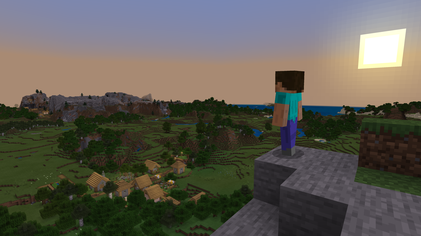
\includegraphics[width=0.75\linewidth]{Minecraft_explore_landscape.png}
\caption{A screenshot of a typical Minecraft world taken from Mojang Studios. Image downloaded from \url{https://en.wikipedia.org/wiki/File:Minecraft_explore_landscape.png} in December 2020.}
\label{fig:minecraft}
\end{figure}

\section{Problem Background}

While generating deformable terrain is the ultimate goal, the main challenge is the extraction of a surface from an area of interest in 3D space~\cite{bourke}. The first step is to identify the location of this region and its bounds. Within this region, it is possible to consider a segment of a scalar field which defines a scalar value at every point in space. This scalar field can be represented by any function $f(x,y,z)$ which returns a scalar value for the input coordinates~\cite{kieran}. Because computers cannot represent this field with infinite fidelity, the scalar field function can be sampled within the region of interest at regular intervals~\cite{kieran}. If an isovalue is then selected, the points in space where the scalar field function equals that isovalue will define an isosurface—a region of constant density~\cite{kieran,lorensen}.\footnote{Changing the isovalue will in turn change the isosurface that is defined~\cite{kieran}.} The task of the marching cubes algorithm is to approximate an isosurface using a given isovalue and the scalar values of the grid~\cite{kieran,bourke}.

To simplify this task, the marching cubes algorithm uses a divide-and-conquer approach~\cite{lorensen,kieran}. Because the scalar field is considered on a structured, uniform grid, each set of eight points makes up the vertices of a logical cube~\cite{lorensen}. The key optimization made by the algorithm is the use of lookup tables. Each vertex is associated with a position in an 8-bit index, with that position being set depending on whether the given vertex is above or below the isosurface~\cite{lorensen,kieran,bourke}. In other words, the index describes the configuration of the current cube. This index is mapped to a particular triangulation using a case-table~\cite{lorensen,kieran,bourke}. The next cube is then “marched,” creating a full mesh when the entire grid has been considered. In this way, the geometry of a cube in the grid is not actually affected by its neighbors~\cite{kieran}.

Determining the triangulation of each case, however, presents its own difficulties. Because there are eight vertices per cube, and two states that each vertex can take, there are a total of $2^8 = 256$ possible ways for an isosurface to intersect the cube—and therefore an equal number of possible triangulations~\cite{lorensen,kieran}. While this is a large amount when considered at face-value, the use of complementary and rotational symmetries means that only 15 different configurations need to be calculated manually~\cite{lorensen,kieran}. Figure \ref{fig:cubecases} illustrates each of these configurations.

\begin{figure}[hbt]
\centering
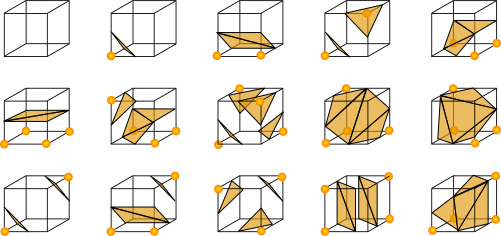
\includegraphics[width=0.75\linewidth]{MarchingCubes.png}
\caption{The original 15 published cases, as represented by Wikipedia user Jmtrivial in 2006. Image downloaded from \url{https://commons.wikimedia.org/wiki/File:MarchingCubes.svg} in December 2020.}
\label{fig:cubecases}
\end{figure}

\section{Related Work}

Originally published by Lorensen and Cline during the proceedings of the 1987 SIGGRAPH conference~\cite{lorensen}, marching cubes is likely the most well known algorithm for extracting a polygonal mesh from a scalar field. It is well documented, and a variety of implementations have been described across different platforms~\cite{lorensen,bourke,bloyd}. The original motivation for the marching cubes algorithm was to improve the visualization of medical data, something that existing techniques struggled to accomplish with high levels of detail~\cite{lorensen}. As Figure \ref{fig:mri} illustrates, the algorithm is capable of handling discrete data produced from MRI scans, CT scans, and other technologies~\cite{lorensen}.

\begin{figure}[hbt]
\centering
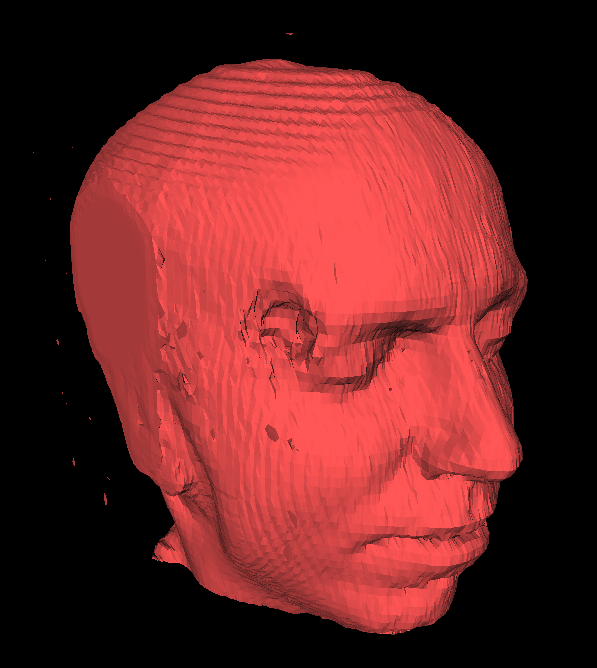
\includegraphics[width=0.50\linewidth]{Marchingcubes-head.png}
\caption{A polygonal mesh extracted from 150 MRI slices using marching cubes, created by Wikipedia user Dake in 2005. Image downloaded from \url{https://commons.wikimedia.org/wiki/File:Marchingcubes-head.png} in December 2020.}
\label{fig:mri}
\end{figure}

The authors also describe several enhancements to the algorithm. Of particular relevance is the use of linear interpolation to place vertices on intersected edges~\cite{lorensen}. While it would be possible to simply place vertices at the midpoint of intersected edges each time, this results in a blockier mesh. Although linear interpolation assumes that the values in the scalar field always change linearly, it still produces a smoother mesh that better approximates the original isosurface. As Sockalingam~\cite{kieran} observes, the interpolation does not interfere with how these vertices are connected to each other; connections depend only on the state of each vertex with regards to being above or below the isosurface.

While Lorensen and Cline focused on the visualization of existing datasets, my project seeks to produce the scalar field from a function as described by Sockalingam and Bourke~\cite{kieran,bourke}. This scalar field function will in turn generate a surface that resembles real terrain. Furthermore, although the original paper discusses solid modeling as a functional enhancement to the marching cubes algorithm~\cite{lorensen}, attention remains for the most part on the static representation of data. Sockalingam~\cite{kieran} notes that the speed of marching cubes makes it suitable for real-time environments, even if the mesh is regenerated every frame. My project aims to leverage this quality to make the extracted mesh truly interactive.

\section{Approach}

The creation of 3D terrain that can be deformed in real time requires two key components. The first is the representation of the terrain itself. Given the discussion of scalar field functions and their role in isosurface extraction, I intended to find an appropriate function to use for sampling. While the extraction process itself does not change based on the sampled values,\footnote{Indeed, as described in the problem background any function at all could be used. The only requirement for the marching cubes algorithm is that a scalar value is defined for every point in the grid.} the focus on terrain specifically led me towards functions that could approximate natural landscapes.

The other component—and arguably the one most important for interactivity—is the treatment of the grid points that sample the scalar field. This meant converting grid points into dynamic entities that could respond to input. If the user is then given a way to change the scalar values within a region of the grid, the extracted surface could change interactively. By regenerating the mesh each time a value change is detected within the grid, any deformation would appear to occur in real time.

\section{Implementation}

In the following subsections, I will explain the implementation process and describe each component of the final application.

\subsection{Tool Selection}

With visualization and user interaction at the core of my project, the choice of development environment was critical. Game engines are a natural fit, because they provide a framework that is well-suited to handling complex graphics and user input. In particular, the Unity game engine was selected for its ease-of-use during development. Unity is arguably one of the most popular game engines that is available for free use, and its rich documentation is supplemented by a large and active community online. The use of C\# for scripting meant that I could easily transfer my prior experience with Java and other—syntactically-similar—programming languages. Finally, and perhaps most importantly, Unity is multi-platform. This meant that I could use the same assets to build executables for Windows, Mac, and Linux.

The actual code for the project was written using Visual Studio, a complete integrated development environment by Microsoft that is bundled with Unity. Git was used to version-control all project assets, while GitHub was used to synchronize the repository across multiple devices.

\subsection{Scalar Field Representation}

The selection of the scalar field function ultimately determines the surfaces that can be extracted. To this end, I wanted to find a noise function that could reliably produce natural-looking terrain. Unity includes its own implementation of Perlin noise with the function \texttt{Mathf.PerlinNoise}~\cite{unityperlin}, which takes a 2D coordinate and returns a value between 0.0 and 1.0. The strength of Perlin noise is that it is pseudo-random; the values at each coordinate change in a gradual way~\cite{unityperlin}. This results in a gradient that is far more natural than pure noise, making the function appropriate for terrain generation.

To actually use Perlin noise, it was also necessary to consider the representation of the grid that would sample the scalar field. In the final implementation, a \texttt{GridPoint} class was constructed that tracks the position and value of a single point in the grid. The grid itself is simply a 3D array of these \texttt{GridPoints}. When the grid is first initialized, or alternately when the user presses the \keystroke{R} key, the scalar field is sampled for each point in the grid. As Listing \ref{lst:perlin} illustrates, this is accomplished by iterating over the entire grid and calling \texttt{Mathf.PerlinNoise} each time.

\begin{listing}[H]
\linespread{1.0}
\caption{Sampling a scalar field created with Perlin noise.}
\begin{minted}[frame=lines]{csharp}
grid[x, y, z].Value = Mathf.PerlinNoise(x, z) * y;
\end{minted}
\label{lst:perlin}
\end{listing}

Because Unity's implementation of Perlin noise is limited to a 2D plane~\cite{unityperlin}, it was necessary to multiply the value returned by \texttt{Mathf.PerlinNoise} by the y-component of the current point. Additionally, in order to account for the scale of the grid as selected in the Unity editor,\footnote{The final application uses a zoom level of 3.0.} each component is divided by the size of the grid in that direction and then multiplied by the selected zoom level. These new values are what is actually used in the final sampling code. Listing \ref{lst:zoom} illustrates this transformation.

\begin{listing}[H]
\linespread{1.0}
\caption{Accounting for grid scale during sampling.}
\begin{minted}[linenos,frame=lines]{csharp}
float nx = Zoom * (x / GridSize.x);
float ny = Zoom * (y / GridSize.y);
float nz = Zoom * (z / GridSize.z);
\end{minted}
\label{lst:zoom}
\end{listing}

In the interactive demo, this process gives the appearance of a flat plane that has been displaced on the y-axis in order to create hills. Of note, Perlin noise will return the same value if given identical coordinates. To produce different terrain each time, a pseudorandom seed is generated before sampling. This seed is added to each component passed to \texttt{Mathf.PerlinNoise}, effectively sampling from a different region of the gradient each time. A more sophisticated use of Perlin noise might layer additional layers of noise at different frequencies, creating finer details, or extend Unity's implementation to three dimensions to create more complex geometry.

To decrease visual ambiguity, the bounds of the grid are visualized during program execution. Unity provides the \texttt{LineRenderer} class~\cite{unityline}, which takes an array of at least two points and draws straight lines between each one. To draw the grid boundaries, a \texttt{LineRenderer} instance is created on startup. Its points are then set in sequence to match the corners of the grid volume.

\subsection{Case-Table Selection}

As explained in the problem background, the marching cubes algorithm is dependent on lookup tables to handle each possible configuration. In this sense, these tables are arguably just as important as the algorithm itself. While Lorensen and Cline reduce the number of cases that need to be computed manually to 15~\cite{lorensen,kieran}, this still presented a significant barrier to actually using marching cubes in my project. To ensure the correctness of my own implementation, I decided to use the triangulation tables created by Bloyd~\cite{bloyd} and later reused by Bourke~\cite{bourke}. 

As explained by Bourke~\cite{bourke}, the first table (called \texttt{edgeTable} in my implementation) is a 256-element array of numbers. The table takes an index representing the current cube configuration and maps it to a single 12-bit number represented in hexadecimal. This number in turn describes which edges of the cube are intersected by the isosurface, with each bit corresponding to the state of a single edge~\cite{bourke}.

The second table (called \texttt{triangleTable} in my implementation), is a 2D array. Like the previous table, the index representing the current configuration is used as a pointer into the array~\cite{bourke}. However, here the index maps to a 16-element integer array that describes the specific triangulation of the intersected points~\cite{bloyd,bourke}. Each triangle is represented by three consecutive integers, with each integer corresponding to the intersected point of a specific edge~\cite{bloyd}. Because some configurations contain less triangles than others, the end of a sequence is marked by the value -1 when necessary~\cite{bloyd}.

\subsection{Algorithm Implementation}

My implementation of the marching cubes algorithm is contained within a single script, called \texttt{MarchingCubes.cs}, but it required additional logic before it could be used in my project. To accomplish this, another script called \texttt{Generate.cs} was created. Apart from handling some user input, the code in this file is what actually drives the bulk of the final application. This includes initializing the grid on startup, sampling the scalar field function, running the marching cubes algorithm, and building the final mesh.

Unity allows for the programmatic creation and modification of meshes through the \texttt{Mesh} class~\cite{unitymesh}. At a minimum, mesh creation requires a set of vertices and a set of triangles that will ultimately form the basic geometry~\cite{unitymesh}. To represent both vectors and positions in 3D space, Unity uses the \texttt{Vector3} structure~\cite{unityvector}. For the \texttt{Mesh} class, vertices are stored as an array of \texttt{Vector3} instances~\cite{unitymesh}. Another array contains a sequence of integers that describe the triangles used for the mesh, with each integer serving as an index into the vertex array~\cite{unitymesh}. In \texttt{Generate.cs}, a new \texttt{Mesh} is obtained every time the isosurface is extracted from the scalar field. As the marching cubes algorithm iterates over every cell in the grid, it determines the necessary vertices and triangles for the current configuration. These are then added to a master vertex and triangle list, which then sets the geometry of the final mesh.

This operation, however, also required thinking about the communication between my marching cubes implementation and \texttt{Generate.cs}. Because the marching cubes algorithm works on one logical cube at a time, it was necessary to package the required information before performing any necessary operations. The \texttt{MarchingCubes.cs} script defines two additional classes that make this possible. The first is a simple \texttt{Triangle} class, which consists of three \texttt{Vector3} instances defining the vertices of a single triangle in 3D space. The second class, \texttt{GridCell}, is more involved and supplements the \texttt{GridPoint} class described earlier. The \texttt{GridCell} class maintains an array of eight \texttt{GridPoints}, an array of \texttt{Triangles}, and an array of \texttt{Vector3} instances that are used to form each triangle for the current configuration.

A single instance of the \texttt{GridCell} class is used by \texttt{Generate.cs}. When the isosurface is extracted or re-extracted by the application, every point of the grid is iterated over. Using the coordinates of each point, the seven other vertices that make up a single cube can also be found. With this information, the vertices of the \texttt{GridCell} instance can be set to the corresponding \texttt{GridPoints}. The marching cubes implementation in \texttt{MarchingCubes.cs} provides a single access point, the function \texttt{Triangulate}, that performs all necessary computation. Once the corners of the cube are defined, a reference to the associated \texttt{GridCell} and the selected isolevel are passed to the function for triangulation.

The marching cubes algorithm, as discussed in the problem background, first requires an index to be computed for use with the lookup tables. Lorensen and Cline~\cite{lorensen} describe an 8-bit index, with each bit corresponding to the state of a particular vertex. However, they do not specify the exact format. In my implementation, a single integer is used to represent the index. While the \texttt{int} type in C\# defaults to a signed 32-bit integer~\cite{integer}, the extra information can simply be ignored when indexing into each table. While other index representations are possible,\footnote{It is worth noting that C\# provides the \texttt{BitArray}~\cite{bitarray} class specifically for managing bit values, and it would also be possible to use a \texttt{bool} array. More work is needed to determine if either approach provides any meaningful space or performance benefits.} their usage would be identical.

Listing \ref{lst:index} illustrates the logic used to find the index. Each \texttt{GridPoint} is checked to determine if its value is less than the given isovalue, which signifies that it is inside the surface. If it is, the corresponding bit is set in the index before considering the next \texttt{GridPoint}. While it would be possible to unroll the loop and perform this check manually for each vertex, using a for-loop improved the conciseness of the final code. Of note is the use of two bitwise operations in the expression \mintinline{csharp}{index |= 1 << i} to actually set the correct bit. The value 1 is shifted left a number of positions equal to \texttt{i}, which accommodates the current value of the loop control variable. When the exclusive-or of this operand and \texttt{index} is taken, this effectively sets the bit at the appropriate position.

\begin{listing}[H]
\linespread{1.0}
\caption{Calculating the index for the current configuration.}
\begin{minted}[linenos,frame=lines]{csharp}
int index = 0;
for (int i = 0; i < 8; i++)
{
    if (cell.p[i].Value < isolevel)
    {
        index |= 1 << i;
    }
}
\end{minted}
\label{lst:index}
\end{listing}

Once the index has been calculated, it is necessary to find where the isosurface meets each intersected edge in the cube. This information will later be used to construct the triangles needed for the current configuration. In order to determine which edges are intersected, the first of Bloyd's~\cite{bloyd} lookup tables is used. Once an intersected edge has been identified, linear interpolation is used to estimate the actual point of intersection along the edge. Finally, the intersection point is added to the \texttt{GridCell} at the corresponding position. Listing \ref{lst:intersection} illustrates this operation.

\begin{listing}[H]
\linespread{1.0}
\caption{Calculating the intersection point for each edge in the cube.}
\begin{minted}[linenos,frame=lines]{csharp}
if (edgeTable[index] == 0) return;
for (int i = 0; i < 12; i++)
{
    if ((edgeTable[index] & (1 << i)) != 0)
    {
        cell.edgepoints[i] = 
        Interpolate(cell.p[vertexTable[i, 0]], 
                          cell.p[vertexTable[i, 1]], 
                          isolevel);
    }
}
\end{minted}
\label{lst:intersection}
\end{listing}

Because this table provides the intersection data in the form of a 12-bit number, a bitwise operation similar to that used in the index calculation is required. Additionally, a check is made before the for-loop is entered. This simply returns if the \texttt{GridCell} is not intersected at any edge, which will occur if every vertex is either above or below the isosurface. In other words, the configuration would not require triangulating. The actual interpolation is performed in a separate function, \texttt{Interpolate}, which takes a pair of \texttt{GridPoints} forming a single edge as well as the selected isovalue. The linear interpolation between two points, $a$ and $b$, can be calculated with the expression $a + (b-a) \cdot t$ where $t$ represents a percentage. This can be translated into C\# relatively simply, as Listing \ref{lst:interpolate} illustrates with the code for \texttt{Interpolate}.

\begin{listing}[H]
\linespread{1.0}
\caption{Interpolating the intersection of a single edge.}
\begin{minted}[linenos,frame=lines]{csharp}
public static Vector3 Interpolate(GridPoint p1, GridPoint p2, float isolevel)
{
    float t = (isolevel - p1.Value) / (p2.Value - p1.Value);
    return p1.Position + t * (p2.Position - p1.Position);
}
\end{minted}
\label{lst:interpolate}
\end{listing}

While Unity does offer the function \texttt{Vector3.Lerp}, which linearly interpolates between two \texttt{Vector3} instances~\cite{unitylerp}, I ultimately decided against using it. The interpolation logic shown above is contained within a single function, which improved readability and testing during development. Additionally, Unity's implementation would still require a separate calculation for the interpolant $t$.

Originally, the task of finding the intersection points was hard-coded, with twelve separate calls to the \texttt{Interpolate} function. Each function call manually provided the two \texttt{GridPoints} that form each edge in the cube. However, in order to convert this operation into a single for-loop, an additional table was added. This table, called \texttt{vertexTable}, uses a list of vertex pairs from Bloyd's implementation~\cite{bloyd} that each represent a particular edge. With this table, the interpolation code can simply look up the required vertices and then pass the associated \texttt{GridPoints} to the \texttt{Interpolate} function.

The final step in the marching cubes algorithm is the construction of each triangle needed for the current configuration. The same index is used, but now as a pointer into Bloyd's~\cite{bloyd} second lookup table. This table, as explained earlier, describes the triangles as a sequence of integers. These integers in turn describe which edges the vertices of the triangles are on. Listing \ref{lst:triangulation} illustrates how each triangle is constructed.

\begin{listing}[H]
\linespread{1.0}
\caption{Constructing each triangle from the intersection points.}
\begin{minted}[linenos,frame=lines]{csharp}
int numTriangles = 0;
for (int i = 0; triangleTable[index, i] != -1; i += 3)
{
    cell.triangles[numTriangles].p[0]
        = cell.edgepoints[triangleTable[index, i]];
    cell.triangles[numTriangles].p[1]
        = cell.edgepoints[triangleTable[index, i + 1]];
    cell.triangles[numTriangles].p[2]
        = cell.edgepoints[triangleTable[index, i + 2]];
    numTriangles++;
}
\end{minted}
\label{lst:triangulation}
\end{listing}

The for-loop iterates over the table until the end of the integer sequence, which is marked by the value -1. A single triangle is built during each iteration. This requires accessing the correct \texttt{Triangle} within the \texttt{GridCell} three times. Each access sets a vertex in the \texttt{Triangle} to the intersection point whose corresponding edge matches the current integer in the sequence. Once this operation is completed for every triangle, the algorithm ends. The \texttt{GridCell} has been successfully triangulated, and the next cube can now be marched.

\subsection{User Interaction}

While the marching cubes algorithm is at the core of my project, the most important feature is how it is ultimately used. In order to let the user deform the extracted isosurface in real time, the algorithm had to be run dynamically. This required enhancing the \texttt{GridPoint} class to accommodate changes in the scalar field. Originally, the \texttt{GridPoint} class was a part of the marching cubes implementation. It simply contained a value and a \texttt{Vector3} that marked its position in the grid. However, in order to make \texttt{GridPoints} dynamic, more integration with the Unity game engine was required. 

In the file \texttt{GridPoint.cs}, the class was redefined to inherit from \texttt{MonoBehaviour}. All Unity scripts derive from this base class~\cite{unitymono}, allowing communication with the game engine. By inheriting from \texttt{MonoBehaviour}, the \texttt{GridPoint} class could be attached as a component and react to the main game loop. When \texttt{Generate.cs} initializes the grid, it creates an empty game object at every point and attaches both a \texttt{GridPoint} instance and a collider. 

If any of the game objects detects a collision, the associated \texttt{GridPoint} checks if the user wants to add to its scalar value or subtract from it. Regardless of the direction, the change is made with respect to the time difference from the last frame. This ensures that any change in value is independent of the frame rate. In addition, the value of the \texttt{GridPoint} is always clamped between 0.0 and 1.0. Restricting the scalar value means that a change to it can be reversed in a short amount of time, preventing the deformation process from feeling too slow.

If the value of a \texttt{GridPoint} is changed, the isosurface needs to be re-extracted from the scalar field. This is handled through a C\# event, which is declared in the \texttt{GridPoint} class and delegated to \texttt{Generate.cs}. Any value change will trigger the event, which sets a flag in \texttt{Generate.cs} to regenerate the mesh. This operation will be carried out in the next frame if the flag is set, which helps prevent repeated build calls from stacking.

While this logic allows for real-time deformation, the user still needs a way to actually interact with the terrain. To solve this problem, I introduced the concept of a “brush.” This brush consisted of a sphere primitive, a translucent material, and a collider slightly larger than the actual object. By locking the brush's position to a fixed distance from the main camera, it would always remain in view as the user moved and looked around the scene. The left and right mouse buttons, when pressed, set flags that add and subtract values in the region defined by the collider. When the user is not pressing either button, the brush's collider is disabled to prevent interaction with the grid. In effect, the brush can be used to seamlessly edit the terrain.

To enable the user to look and move around, I adapted a script posted by user IJM~\cite{camera} on the Unity online forum. The script was modified to support using the brush, and the movement controls were also changed to match those seen in Minecraft. As previously mentioned, \texttt{Generate.cs} also handles some user input. When the user presses the \keystroke{R} key to create new terrain, the texture used for the mesh is picked at random from several different options. When the \keystroke{C} key is pressed, every \texttt{GridPoint} is given the value 1.0. This results in no visible mesh, giving the user the entire grid to draw in.

\subsection{Application Deployment}

To make my project available outside of the Unity editor, I used the engine's provided tools to package and export the final application. Versions for both Windows and Mac have been tested, but a Linux build should also be possible. While I intended to host a WebGL build as well, it was not functional outside of basic movement. Further testing is required to determine the source of the problem.

\section{Evaluation}

Because the goal of my project was to use marching cubes interactively, the performance of the algorithm was critical. This concerns the initial triangulation on startup, but also the behavior of the algorithm when the user continuously edits the generated terrain. The primary evaluation was the time required to triangulate the mesh once. More specifically, a number of grid sizes were tested to find how long the algorithm took to triangulate increasingly larger regions of space. C\# provides a \texttt{Stopwatch} class that can be used to accurately measure and record time~\cite{stopwatch}.

In \texttt{Generate.cs}, a \texttt{StopWatch} instance is created every time the mesh is regenerated. After the isosurface is extracted, the elapsed time in milliseconds is printed to the Unity Console. Six grid dimensions were tested, ranging from a $1\times1\times1$ grid to one that was $50\times50\times50$. All tests were run on a desktop computer with an NVIDIA GeForce 1080 Ti graphics card and an Intel Core i5 processor clocked at 3.5GHz. As Table \ref{table:times} illustrates, at no point was more than 100 milliseconds required to triangulate the scalar field.

\begin{table}[hbt]
\centering
\begin{tabular}{|l|l|}
\hline
\textbf{Grid Size} & \textbf{Time (ms)}\\
\hline
\hline
$1\times1\times1$ & < 1\\
\hline
$10\times10\times10$ & 1\\
\hline
$20\times20\times20$ & 6\\
\hline
$30\times30\times30$ & 19\\
\hline
$40\times40\times40$ & 44\\
\hline
$50\times50\times50$ & 83\\
\hline
\end{tabular}
\caption{Time to triangulate mesh once.}
\label{table:times}
\end{table}

It is also worth mentioning the overall frame rate. In general, the application exceeded 2000 frames per second at grid sizes below $30\times30\times30$. Drops to 600 FPS, however, occurred when the mesh was being continuously regenerated by the brush. At larger dimensions, the average frame rate was lowered to double-digits. An interesting observation is that the marching cubes algorithm does not appear to be the main performance bottleneck. Indeed, the larger grid sizes show that it is actually rendering the triangulated mesh that slows the application the most. In my implementation, adjacent cubes are not able to share vertices. This ultimately contributes to the complexity of the mesh growing faster than is necessary. The Unity Editor itself also adds overhead, a fact that likely affected the reported numbers during testing.

\section{Conclusions and Future Work}

The beauty of the marching cubes algorithm is in its simplicity. Because each triangulation is precomputed, most of the work can be accomplished by indexing into the correct lookup table. My project shows that marching cubes is not only viable for real-time applications, but also that it improves the quality of generated terrain. The algorithm remained performant during periods of high utilization, and produced results that were more convincing than a voxel-based approach. I originally wanted to create deformable 3D terrain, and I believe my project has more than succeeded in that goal.

With this success in mind, there is still a wealth of possible work that can and should be explored. My project only touched the surface of this algorithm's potential, and even the focus on terrain specifically could be expanded much further. For one, my use of Perlin noise was relatively limited. More sophisticated approaches to noise generation exist, and they have the potential to create more interesting surfaces with higher levels of detail.

The algorithm itself is also open to improvement. Sockalingam~\cite{kieran} notes that the 15 originally published cases allow for holes between adjacent grid cells. The behavior of the scalar field is also not taken into account during triangulation, which can lead to ambiguities in the final mesh~\cite{kieran}. Expanded implementations of the marching cubes algorithm have attempted to solve these problems~\cite{kieran}, and it would be interesting to evaluate them in the context of real-time applications.

Finally, my marching cubes implementation does not leverage the GPU. Because neighboring cubes do not affect each other's geometry, the algorithm is well-suited to parallel computation~\cite{kieran}. In Unity, it is possible to write compute shaders that will run on the available graphics hardware. The greatest optimization potential is likely here, and a future implementation of marching cubes using compute shaders could drastically improve performance. 

\section*{Acknowledgements}

I graciously thank my adviser, Professor Szymon Rusinkiewicz, for enabling me to undertake this project. It was a privilege to explore an interesting algorithm in such detail, and I am a better computer scientist because of it. I also thank all my friends and family. Their tireless support during the semester made this project possible.

\section*{Honor Code}

I pledge my honor that this paper represents my own work in accordance with University regulations \\/s/ William Svoboda

\pagebreak

\bstctlcite{bstctl:etal, bstctl:nodash, bstctl:simpurl}
\bibliographystyle{IEEEtranS}
\bibliography{references}

\appendix

\section{Appendix}

All project code is hosted on GitHub at \url{https://github.com/disstillwill/IW-Fall-2020} along with links to builds of the final application.

\end{document}

